\documentclass[twoside]{mfitjournal}
\usepackage{amsbib}
\usepackage[T2A]{fontenc}
\usepackage[utf8]{inputenc}
\usepackage[russian]{babel}
\usepackage{amsmath}
\usepackage{graphicx}
\usepackage{geometry}
\usepackage{array}
\usepackage{booktabs}
\usepackage{caption}
\usepackage{float}
\clubpenalty=10000
\widowpenalty=10000
\newcommand{\MFITnumber}{}
\newcommand{\MFITom}{}
\newcommand{\MFITyear}{}
\newcommand{\ISSN}{}
\newcommand{\OISSN}{}
\newcommand{\DOI}{}
\renewcommand{\firstpage}{}
\renewcommand{\lastpage}{}
\SECC{}
\ESECC{}
\geometry{margin=2cm}
\setlength{\headheight}{15pt}
\captionsetup{font=small, labelfont=bf}

\begin{document}

\rustitle{Лабораторная работа 4.3.6. Дифракция света на периодических структурах}
\shorttitle{Лабораторная работа 4.3.6}
\author{Евгений Иванов}
\shortauthor{Иванов Е.\,И.}
\institute{МФТИ, группа 5-407}
\email{E-mail:}{}
\rcopyr{Евгений Иванов}

\makeatletter
\renewcommand{\tit}{}
\renewcommand{\@oddhead}{}
\renewcommand{\@evenhead}{}
\makeatother

\pagestyle{fancy}
\fancyhf{}
\fancyhead[RE]{Иванов Е.\,И.}
\fancyhead[LO]{Лабораторная работа 4.3.6}
\cfoot{\arabic{page}}

\maketitle

\section*{Цель работы}

Изучить дифракцию света на периодических структурах и эффект саморепродукции Талбота, а также определить периоды двумерных сеток по спектру, по увеличенному изображению и по координатам плоскостей саморепродукции.

\section*{Оборудование и установка}

В работе использовались зелёный лазер с длиной волны $\lambda = 530$ нм, кассета с двумерными сетками, короткофокусная линза с микрометрическим винтом, экран и линейка. Лазерное излучение падало практически нормально на сетку.

\section*{Краткая теория}

Дифракция возникает тогда, когда волновую природу света уже нельзя пренебречь. Поле за решёткой удобно рассматривать как сумму плоских волн, идущих под разными углами. Для периодической структуры это эквивалентно разложению по Фурье, поэтому её пространственный спектр состоит из отдельных гармоник.

На экране наблюдается картина спектра. Для решётки это набор узких максимумов.

Для двумерной квадратной сетки условия максимумов имеют вид
\begin{equation}
d\sin\theta_x = m_x\lambda, \qquad d\sin\theta_y = m_y\lambda,
\end{equation}
где $d$ --- период сетки, $m_x$ и $m_y$ --- порядки максимумов. В работе использовались малые углы, поэтому
\begin{equation}
\sin\theta \approx \theta \approx \frac{x}{L},
\end{equation}
где $x$ --- расстояние между соседними максимумами, $L$ --- расстояние от сетки до экрана. Отсюда
\begin{equation}
d_{\text{сп}} = \frac{\lambda L}{x}.
\end{equation}

Если поле сразу за решёткой представить в виде ряда Фурье
\begin{equation}
f_0(x) = \sum\limits_n c_n e^{i 2\pi n x/d},
\end{equation}
то после прохождения расстояния $z$ каждая гармоника получает свой фазовый множитель, и поле можно записать как
\begin{equation}
f(x,z) = \sum\limits_n c_n e^{i 2\pi n x/d}\exp\left(-i\pi\frac{\lambda z}{d^2}n^2\right).
\end{equation}
Из этой формулы видно, что саморепродукция связана именно с повторным совпадением фаз всех пространственных гармоник.

Линза в этой работе использовалась для получения увеличенного изображения сетки. Кроме того, её фокальная плоскость является фурье-плоскостью, в которой собираются дифракционные максимумы. Это соответствует обычной схеме Аббе: сначала формируется спектр, а затем по нему строится изображение.

Если сетка наблюдается в режиме геометрического изображения, то при расстояниях $a$ от линзы до сетки и $b$ от линзы до экрана коэффициент увеличения равен $b/a$, поэтому
\begin{equation}
d_{\text{л}} = D\frac{a}{b},
\end{equation}
где $D$ --- размер клетки в изображении на экране.

В области френелевской дифракции для периодических структур наблюдается эффект Талбота. При распространении разные гармоники набирают разные фазы, и на некоторых расстояниях их относительные фазы снова совпадают с исходными (см лабник). В этих плоскостях изображение решётки воспроизводится. Полные плоскости саморепродукции расположены на расстояниях
\begin{equation}
z_m = m\frac{2d^2}{\lambda}, \qquad m = 1,2,\ldots
\end{equation}
Отсюда период можно определить как
\begin{equation}
d_{\text{реп}} = \sqrt{\frac{z_m\lambda}{2m}}.
\end{equation}

Одиночная проволочка не является периодическим объектом и потому не репродуцируется; именно это позволяет использовать кассету с проволочкой для поиска настоящего геометрического изображения.

\section*{Методика измерений}

Сначала для каждой кассеты без линзы измерялось расстояние $X$ между удалёнными максимумами на экране (через центр) и по числу промежутков $n$ вычислялось расстояние между соседними максимумами:
\begin{equation}
x = \frac{X}{n}.
\end{equation}

Во второй части с линзой получалось увеличенное изображение сетки на экране. На листе бумаги отмечался отрезок длиной $\ell$, покрывающий несколько интервалов сетки. Если число интервалов равно $N$, то
\begin{equation}
D = \frac{\ell}{N}.
\end{equation}

В третьей части по нониусной шкале микровинта измерялись положения резких изображений сетки. За нулевой уровень отсчёта принималось геометрическое изображение при показании (см фотографию)
\begin{equation}
s_0 = 5.0\ \text{см}.
\end{equation}
Затем для каждого резкого изображения записывался отсчёт $s_N$, который снимался по вертикальной отметке корпуса (см фото). Соответствующее смещение вычислялось как
\begin{equation}
z_N = (s_0 - s_N)\cdot 10\ \text{мм}.
\end{equation}

\begin{figure}[H]
\centering
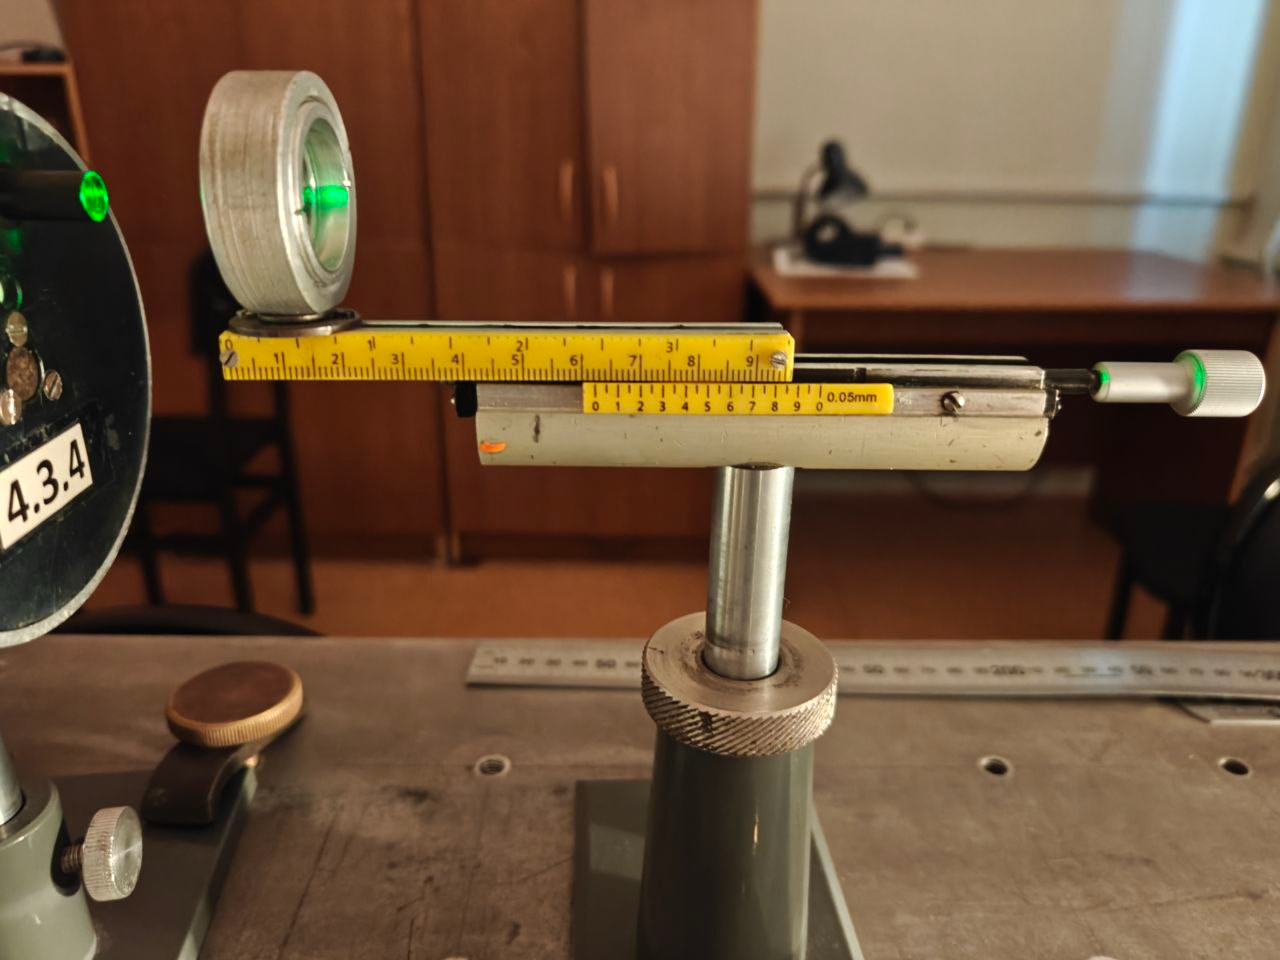
\includegraphics[width=0.70\textwidth]{photos/Pasted image (7).png}
\caption{Отсчёт по шкале микровинта. Значение снималось по вертикальной риске корпуса.}
\end{figure}

При обработке саморепродукции все наблюдавшиеся резкие изображения нумеровались по порядку появления: $N=1,2,\ldots$ Для каждой кассеты строился график $z_N(N)$ и проводилась линейная аппроксимация
\begin{equation}
z_N = kN + b.
\end{equation}
и по коэфициенту наклона вычислялось $d$.

\section*{Экспериментальные данные}

Исходные параметры установки:
\[
\lambda = 530\ \text{нм}, \qquad L = (1060 \pm 10)\ \text{мм},
\]
\[
a = (60 \pm 10)\ \text{мм}, \qquad b = (1300 \pm 20)\ \text{мм}.
\]

\subsection*{1. Спектральный метод}

\begin{table}[H]
\centering
\caption{Измеренные величины для спектрального метода}
\begin{tabular}{ccccc}
\toprule
Кассета & $X$, мм & $\Delta X$, мм & $n$ & $x = X/n$, мм \\
\midrule
K1 & 194 & 5 & 6  & 32.333 \\
K2 & 127 & 5 & 6  & 21.167 \\
K3 & 127 & 5 & 12 & 10.583 \\
K4 & 85  & 5 & 16 & 5.312 \\
K5 & 80  & 5 & 20 & 4.000 \\
\bottomrule
\end{tabular}
\end{table}

\subsection*{2. Линзовый метод}

\begin{table}[H]
\centering
\caption{Измеренные величины для линзового метода}
\begin{tabular}{ccccc}
\toprule
Кассета & $\ell$, мм & $\Delta \ell$, мм & $N$ & $D = \ell/N$, мм \\
\midrule
K3 & 13 & 2 & 11 & 1.182 \\
K4 & 15 & 2 & 7  & 2.143 \\
K5 & 35 & 2 & 21 & 1.667 \\
\bottomrule
\end{tabular}
\end{table}

\subsection*{3. Саморепродукция}

\begin{table}[H]
\centering
\caption{Отсчёты по микровинту и соответствующие им смещения}
\begin{tabular}{p{1.4cm}p{5.0cm}p{4.8cm}}
\toprule
Кассета & $s_N$, см & $z_N$, мм \\
\midrule
K3 & $4.6;\ 4.3;\ 4.0;\ 3.6;\ 3.3;\ 3.0$ & $4;\ 7;\ 10;\ 14;\ 17;\ 20$ \\
K4 & $4.3;\ 3.7;\ 2.7;\ 0.0$ & $7;\ 13;\ 23;\ 50$ \\
K5 & $3.25;\ 0.5;\ -1.75$ & $17.5;\ 45.0;\ 67.5$ \\
\bottomrule
\end{tabular}
\end{table}

Погрешность каждого отсчёта по микровинту принималась равной $\pm 0.2$ см, то есть $\Delta z = \pm 2$ мм.

\section*{Обработка результатов}

\subsection*{1. Периоды по спектру}

Погрешность вычислялась по формуле
\begin{equation}
\frac{\Delta d_{\text{сп}}}{d_{\text{сп}}}
=
\sqrt{
\left(\frac{\Delta L}{L}\right)^2 +
\left(\frac{\Delta x}{x}\right)^2
}.
\end{equation}

\begin{table}[H]
\centering
\caption{Результаты спектрального метода}
\begin{tabular}{ccc}
\toprule
Кассета & $d_{\text{сп}}$, мкм & $z_T^{(\text{сп})}$, мм \\
\midrule
K1 & $17.4 \pm 0.5$ & 1.14 \\
K2 & $26.5 \pm 1.1$ & 2.66 \\
K3 & $53.1 \pm 2.1$ & 10.63 \\
K4 & $105.8 \pm 6.3$ & 42.20 \\
K5 & $140.5 \pm 8.9$ & 74.44 \\
\bottomrule
\end{tabular}
\end{table}

\subsection*{2. Периоды по увеличенному изображению}

\begin{equation}
\frac{\Delta d_{\text{л}}}{d_{\text{л}}}
=
\sqrt{
\left(\frac{\Delta D}{D}\right)^2 +
\left(\frac{\Delta a}{a}\right)^2 +
\left(\frac{\Delta b}{b}\right)^2
}.
\end{equation}

\begin{table}[H]
\centering
\caption{Результаты линзового метода}
\begin{tabular}{cc}
\toprule
Кассета & $d_{\text{л}}$, мкм \\
\midrule
K3 & $54.5 \pm 12.4$ \\
K4 & $98.9 \pm 21.2$ \\
K5 & $76.9 \pm 13.6$ \\
\bottomrule
\end{tabular}
\end{table}

\subsection*{3. Периоды по саморепродукции}

Для всех трёх кассет были построены графики $z_N(N)$ и на каждом графике проведена линейная аппроксимация.

\begin{figure}[H]
\centering
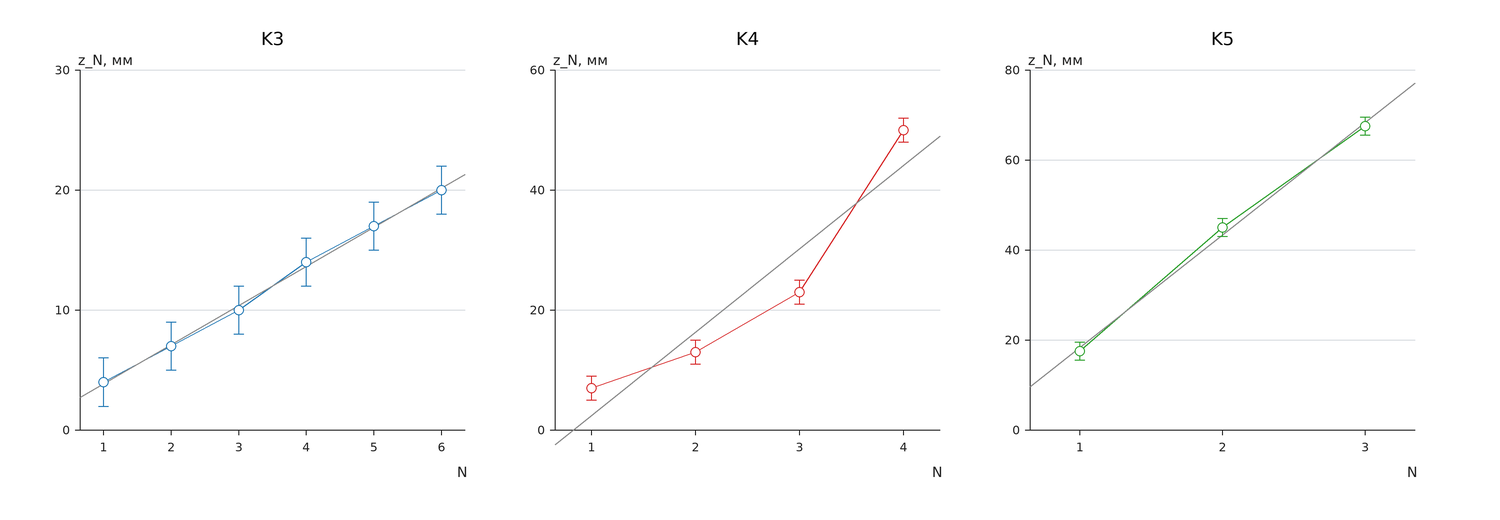
\includegraphics[width=\textwidth]{all_self_reproduction_points.png}
\caption{Графики $z_N(N)$ для кассет $K3$, $K4$ и $K5$. Серой линией показана линейная аппроксимация.}
\end{figure}

Если формально считать, что наклон $k$ задаёт расстояние между соседними репродуцированными изображениями, то период находится по формуле
\[
d_{\text{реп}} = \sqrt{\frac{k\lambda}{2}}.
\]

Погрешность вычислялась из соотношения
\begin{equation}
\frac{\Delta d_{\text{реп}}}{d_{\text{реп}}} = \frac{1}{2}\frac{\Delta k}{k}.
\end{equation}

\begin{table}[H]
\centering
\caption{Линейная аппроксимация графиков $z_N(N)$ и формальные значения $d_{\text{реп}}$}
\begin{tabular}{ccccc}
\toprule
Кассета & $k$, мм & $b$, мм & $R^2$ & $d_{\text{реп}}$, мкм \\
\midrule
K3 & $3.26 \pm 0.07$ & $0.6 \pm 0.3$ & 0.998 & $29.4 \pm 0.3$ \\
K4 & $13.9 \pm 3.4$ & $-11.5 \pm 9.4$ & 0.891 & $60.7 \pm 7.5$ \\
K5 & $25.0 \pm 1.4$ & $-6.7 \pm 3.1$ & 0.997 & $81.4 \pm 2.3$ \\
\bottomrule
\end{tabular}
\end{table}

\subsection*{4. Сводная таблица}

\begin{table}[H]
\centering
\caption{Сравнение результатов разных методов}
\begin{tabular}{cccc}
\toprule
Кассета & $d_{\text{сп}}$, мкм & $d_{\text{л}}$, мкм & $d_{\text{реп}}$, мкм \\
\midrule
K1 & $17.4 \pm 0.5$ & --- & --- \\
K2 & $26.5 \pm 1.1$ & --- & --- \\
K3 & $53.1 \pm 2.1$ & $54.5 \pm 12.4$ & $29.4 \pm 0.3$ \\
K4 & $105.8 \pm 6.3$ & $98.9 \pm 21.2$ & $60.7 \pm 7.5$ \\
K5 & $140.5 \pm 8.9$ & $76.9 \pm 13.6$ & $81.4 \pm 2.3$ \\
\bottomrule
\end{tabular}
\end{table}

\section*{Обсуждение результатов}

Для кассеты $K3$ линейная аппроксимация по всем шести резким изображениям даёт
\[
d_{\text{реп}} = (29.4 \pm 0.3)\ \text{мкм},
\]
тогда как по спектру и по линзе получается около $53$--$55$ мкм. Расхождение сильное, почти в полтора два раза.

Для кассеты $K4$ по спектру и по линзе получается примерно $100$ мкм, а формальная аппроксимация даёт только
\[
d_{\text{реп}} = (60.7 \pm 7.5)\ \text{мкм}.
\]
На графике отклоняются от прямой, коэффициент детерминации всего навсего $R^2 = 0.891$. Результат по саморепродукции для этой нельзя считать надёжным. Наверное косяк с измерениями

Для кассеты $K5$ формально получается
\[
d_{\text{реп}} = (81.4 \pm 2.3)\ \text{мкм},
\]
что близко к результату линзового метода $76.9 \pm 13.6$ мкм, но также расходятся со спектральным значением $140.5 \pm 8.9$ мкм.

Условие дифракции Фраунгофера в работе выполнено. Для самой крупной сетки
\[
\frac{d^2}{\lambda} \approx \frac{(140\ \text{мкм})^2}{0.53\ \text{мкм}} \approx 37\ \text{мм},
\]
что значительно меньше расстояния до экрана $L=1060$ мм.

\section*{Заключение}

В работе были исследованы дифракция света на периодических структурах. Периоды сеток определялись по спектру, по увеличенному изображению и по координатам резких изображений при саморепродукции.

Наиболее надёжные значения получены спектральным методом:
\[
d_{K1} = (17.4 \pm 0.5)\ \text{мкм},\quad
d_{K2} = (26.5 \pm 1.1)\ \text{мкм},
\]
\[
d_{K3} = (53.1 \pm 2.1)\ \text{мкм},\quad
d_{K4} = (105.8 \pm 6.3)\ \text{мкм},\quad
d_{K5} = (140.5 \pm 8.9)\ \text{мкм}.
\]

Формальная линейная обработка всех графиков $z_N(N)$ дала значения
\[
d_{K3}^{(\text{реп})} = (29.4 \pm 0.3)\ \text{мкм},\quad
d_{K4}^{(\text{реп})} = (60.7 \pm 7.5)\ \text{мкм},
\]
\[
d_{K5}^{(\text{реп})} = (81.4 \pm 2.3)\ \text{мкм}.
\]
В данной работе метод саморепродукции требует более точных измерений.

\begin{thebibliography}{99}
\bibitem{labmanual}
Лабораторный практикум по общей физике: учеб. пособие. В 3 т. Т. 2. Оптика / А.\,В. Максимычев, Д.\,А. Александров, Н.\,С. Берюлёва и др.; под ред. А.\,В. Максимычева. М.: МФТИ, 2014. 446 с.
\end{thebibliography}

\end{document}
